\documentclass
% Uncomment to get one page per frame
%[handout]
{beamer}

\usepackage{amsfonts}
\usepackage{amsmath}
\usepackage{longtable}
\usepackage{csquotes}
\usepackage{standalone}

\usepackage{graphicx}
\graphicspath{{../pictures/}}

\usepackage{tikz}
\usetikzlibrary{shapes, calc, arrows, decorations.markings,
  decorations.pathmorphing, decorations, patterns, chains, snakes,
  backgrounds, positioning, fit, petri}
\newcommand{\inputpicture}[1]{\input{../drawings/#1}}

\newcommand{\reg}{\textsuperscript{\textregistered}}

\usepackage{listings}
\lstset{language=C, basicstyle=\ttfamily, breaklines=true, keepspaces=true,
  keywordstyle=\color{blue}}

\usepackage{bytefield}

\usefonttheme{professionalfonts}
\usefonttheme{serif}
\usepackage{fontspec}
\setromanfont{CMU Serif}
\setsansfont{CMU Sans Serif}
\setmonofont{CMU Typewriter Text}

\newcommand{\No}{{\fontfamily{lmr}\selectfont \textnumero}}

\usepackage{hyperref}
\hypersetup{colorlinks=true, linkcolor=black, filecolor=black, citecolor=black,
  urlcolor=blue , pdfauthor=Evgenii Iuliugin <yulyugin@gmail.com>,
  pdftitle=Fundamentals of Full-Platform Simulation}

\usepackage{underscore}
\usepackage{amsthm}

\subtitle{Fundamentals of Full-Platform Simulation}
\subject{Lecture}
\date{\today}

\author[Evgenii Iuliugin]{
  Evgenii Iuliugin, \small{\href{mailto:yulyugin@gmail.com}{yulyugin@gmail.com}}}
\typeout{Copyright 2021 Evgenii Iuliugin}
\institute{Moscow Institute of Physics and Technology}

\usepackage[bibencoding=inputenc, backend=biber, language=auto,
  style=alphabetic]{biblatex}
\addbibresource{../common/virtualization.bib}
\addbibresource{../common/modelling-languages.bib}
\addbibresource{../common/parallel-simulation.bib}

\usetheme{Madrid}
\setbeamertemplate{navigation symbols}{}

\definecolor{miptdark}{RGB}{25,52,104}
\definecolor{miptlight}{RGB}{1,114,192}
\setbeamercolor{author in head/foot}{fg=white, bg=miptlight}
\setbeamercolor{title in head/foot}{fg=white, bg=miptdark}

\makeatletter
\setbeamertemplate{footline}{%
  \leavevmode%
  \hbox{%
    \begin{beamercolorbox}[wd=.15\paperwidth,ht=2.25ex,dp=1ex,center]{author in head/foot}%
      \usebeamerfont{author in head/foot}\insertshortauthor
    \end{beamercolorbox}%
    \begin{beamercolorbox}[wd=.77\paperwidth,ht=2.25ex,dp=1ex,center]{title in head/foot}%
      \usebeamerfont{title in head/foot}\inserttitle
    \end{beamercolorbox}%
  }%
  \begin{beamercolorbox}[wd=.08\paperwidth,ht=2.25ex,dp=1ex,right]{date in head/foot}%
    \usebeamerfont{date in head/foot}%
    \usebeamertemplate{page number in head/foot}%
    \hspace*{2ex}
  \end{beamercolorbox}
  \vskip-1pt%
}
\makeatother

\newcommand{\startslides}{
  {\setbeamertemplate{footline}{}
  \begin{frame}
      \maketitle
  \end{frame}
  }

  \addtocounter{framenumber}{-1}

  \begin{frame}{\inserttitle}
      \tableofcontents
  \end{frame}
}

\newcommand{\finalslide}{{
  \setbeamertemplate{footline}{}

  \begin{frame}

  {\huge{Thank you!}\par}

  \vfill
  Slides and material are available at
  \url{https://github.com/yulyugin/sim-lectures}
  \vfill

  \tiny{\textit{Note}: All trademarks are the property of their respective
    owners. The presented point of view reflects the personal opinion of
    the author.

    %All the materials are licensed under the Creative Commons
    %Attribution-NonCommercial-ShareAlike 4.0 Worldwide. To view a copy of this
    %license, visit \url{http://creativecommons.org/licenses/by-nc-sa/4.0/}.
  }
  \end{frame}
}\addtocounter{framenumber}{-1}}

\title{Hardware Assisted Virtualization}

\begin{document}

\startslides

\begin{frame}{On the Previous Lecture:}
  \begin{itemize}
    \item Cycle-accurate simulation.
    \item Functions and ports.
    \item Approximate timing.
    \item Full speed ahead.
  \end{itemize}
\end{frame}

\begin{frame}{Questions}
  \begin{itemize}
    \item What phases exist in port-based cycle-accurate model?\pause
    \item How many independent inputs can a functional element have?\pause
    \item How many independent inputs can a port have?
  \end{itemize}
\end{frame}

\begin{frame}{Simulation vs. Emulation vs. Virtualization}
\begin{itemize}
\item \textbf{Simulation}\pause --- replication of system's behavior that can
  be observed through \textbf{\textit{external}} interaction with the system.
\item \textbf{Emulation}\pause --- replication of a system's behavior
  considering how the system \textbf{\textit{internally}} works through
  imitation of all internal structures and processes.
\item \textbf{Virtualization}\pause --- effective isolation of several systems
  from each other with simultaneous and transparent access to resources of the
  underlying system.
\end{itemize}
\end{frame}

\begin{frame}{Simulation vs. Virtualization}
\centering
\inputpicture{simulation-levels}
\vfill
\inputpicture{multiplexing}
\end{frame}

\begin{frame}{History}
\begin{itemize}
\item IBM VM --- 1960.
\item VMware Workstation --- 1998.
\item Intel\reg~VT-x --- 2005.
\end{itemize}
\end{frame}

\section{Formal Requirements}

\subsection{Virtual Machine Concept}

\begin{frame}{Definition}
\textit{Gerald J. Popek, Robert P. Goldberg}, ``Formal requirements for
virtualizable third generation
architectures''~\cite{popek-goldberg-vm-requirements}:
\vfill\pause
A \textit{virtual machine} is taken to be an \textbf{efficient},
\textbf{isolated} \textbf{duplicate} of the real machine.
\vfill\pause
\textit{Virtual machine monitor (VMM)} provides:
\begin{enumerate}
\item an environment for programs equivalent to the original machine;\pause
\item programs run in this environment show at worst only minor decreases in
  speed;\pause
\item the VMM is in complete control of system resources.
\end{enumerate}
\end{frame}

\begin{frame}{Properties}
\begin{itemize}
\item \textbf{Equivalent} means that any program running under the
  VMM control should demonstrated identical to the original machine behavior,
  except differences caused by the availability of system resources and
  timing.\pause
\item \textbf{Efficiency} demands that a statistically dominant subset of the
  virtual processor's instructions is executed directly by the real processor,
  with no software intervention by the VMM.\pause
\item \textbf{Resource control}:
  \begin{enumerate}
  \item a program running under VMM cannot access resources not explicitly
    allocated to it;
  \item VMM can regain control of already allocated resources.
  \end{enumerate}
\end{itemize}
\end{frame}

\subsection{Model of Machines}

\begin{frame}{Model of Machines}
\begin{itemize}
\item Single processor executing instructions.
\item The processor's state $(E, M, P, R)$:
  \begin{itemize}
  \item Linear memory $E$ of size $q$, addressing $E[i]$,
  \item Two modes $M$: $u$ (user) and $s$ (supervisor),
  \item Program counter --- $P$,
  \item Memory segment --- $R (l, b)$.
  \end{itemize}
\item Instruction $i(E_1, M_1, P_1, R_1) = (E_2, M_2, P_2, R_2)$.
\end{itemize}
\end{frame}

\begin{frame}{Trap}
An instruction $i$ is trap if:
\begin{equation*}
  \begin{aligned}
  i(E_1, M_1, P_1, R_1) &= (E_2, M_2, P_2, R_2)\text{, where} \\
  E_2[j] &= E_1[j]\text{, for } 0 < j < q, \\
  E_2[0] &= (M_1, P_1, R_1), \\
  (M_2, P_2, R_2) &= E_1[1].
  \end{aligned}
\end{equation*}
\pause\vfill
Trap types:
\begin{enumerate}
\item Control trap --- caused by an attempt to change the processor's state.
\item Memory trap --- caused by an attampt to access an out of bound address.
\end{enumerate}
\end{frame}

\begin{frame}{Instructions}
\begin{itemize}
\item \textbf{Prigileged}: execution with $M=u$ always causes a
  control trap.\pause
\item \textbf{Sensitive}:
  \begin{itemize}
  \item \textit{Control} sensitive instructions change $M$ and/or $R$.
  \item \textit{Behavior} sensitive instructions operate differently depending
    on $M$ or $R$.\pause
  \end{itemize}
  \item \textbf{Innocuous} --- neither privileged nor sensitive.
\end{itemize}
\end{frame}

\subsection{Sufficient Conditions for Virtualizability}

\begin{frame}{Sufficient Conditions for Virtualizability}
A virtual machine monitor may be constructed if the set of sensitive
instructions for that computer is a subset of the set of privileged
instructions.
\vfill\centering
\inputpicture{vm-sufficient-condition} 
\end{frame}

\begin{frame}{Construction}
\begin{enumerate}
\item VMM operates in supervisor mode.
\item VMs operate in user mode:
  \begin{itemize}
  \item innocuous instructions are executed directly,
  \item sensitive instructions cause traps and emulation by the VMM,
  \item privileged instructions cause traps and emulation by the VMM.
  \end{itemize}
\end{enumerate}
\pause
\centering$\Downarrow$
\begin{enumerate}
  \item Isolation,
  \item Equivalence,
  \item Efficiency.
\end{enumerate}
\end{frame}

\section{Modern Adjustments}

\begin{frame}{What Is Missing?}
\begin{itemize}
  \item Complex address translation,
  \item Peripheral devices,
\end{itemize}
\end{frame}

\subsection{Address Translation}

\begin{frame}{Address Translation}
\centering
\inputpicture{two-level-translation} 
\end{frame}

\begin{frame}{TLB for Virtualization}
\begin{center}
\begin{tabular}{rrr}
Virtual address & Physical address & Tag\\
0x11112222000   &  0x22220000      & VM1\\
0x11112222000   &  0x11110000      & VM2\\
0x44443333000   &  0x55554000      & MON\\
0xabcd9876000   &  0x00001000      & VM1\\
0xabcd9876000   &  0x11111000      & VM3
\end{tabular}
\end{center}
\end{frame}

\subsection{Peripheral Devices}

\begin{frame}{Peripheral Devices}
\begin{itemize}
  \item Whom to deliver?
  \item What if interrupts are disabled in a VM?
\end{itemize}
\vfill
\centering
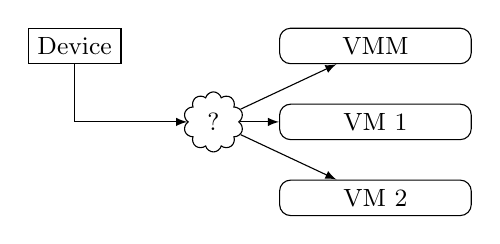
\begin{tikzpicture}[>=latex, font=\small, align=center]
  \node[draw] (dev) {Device};

  \node[draw, rounded corners, right=2cm of dev, text width=2.2cm] (vmm) {VMM};
  \node[draw, rounded corners, below = 0.5 cm of vmm, text width=2.2cm] (vm1) {VM 1};
  \node[draw, rounded corners, below = 0.5cm of vm1, text width=2.2cm] (vm2) {VM 2};

  \node[draw, left=0.5cm of vm1, cloud] (sel) {?};

  \draw[->] (dev) |- (sel);
  \draw[->] (sel) -- (vmm);
  \draw[->] (sel) -- (vm1);
  \draw[->] (sel) -- (vm2);
\end{tikzpicture}
\end{frame}

\begin{frame}{Conservative Approach}
\begin{itemize}
  \item All interrupts delivered to VMM,
  \item VMM injects interrupts to VMs,
\end{itemize}
\vfill
\centering
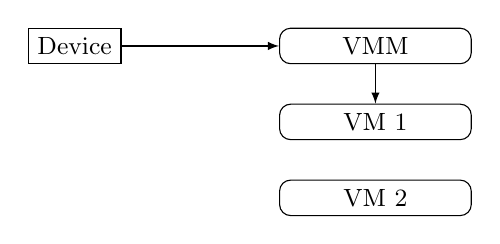
\begin{tikzpicture}[>=latex, font=\small, align=center]
  \node[draw] (dev) {Device};

  \node[draw, rounded corners, right=2cm of dev, text width=2.2cm] (vmm) {VMM};
  \node[draw, rounded corners, below = 0.5 cm of vmm, text width=2.2cm] (vm1) {VM 1};
  \node[draw, rounded corners, below = 0.5cm of vm1, text width=2.2cm] (vm2) {VM 2};

  \draw[->] (dev) -- (vmm);
  \draw[->] (vmm) -- (vm1);
\end{tikzpicture}
\begin{itemize}
  \item Higher interrupt latency.
\end{itemize}
\end{frame}

\begin{frame}{Hardware Support}
\begin{itemize}
  \item Hardware delivers permitted interrupts to VMs,
  \item Other interrupts delivered to VMM.
\end{itemize}
\vfill
\centering
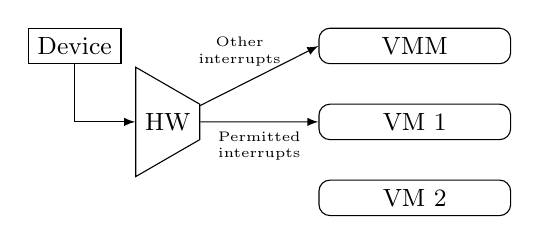
\begin{tikzpicture}[>=latex, font=\small, align=center]
  \node[draw] (dev) {Device};

  \node[draw, rounded corners, right=2.5cm of dev, text width=2.2cm] (vmm) {VMM};
  \node[draw, rounded corners, below = 0.5 cm of vmm, text width=2.2cm] (vm1) {VM 1};
  \node[draw, rounded corners, below = 0.5cm of vm1, text width=2.2cm] (vm2) {VM 2};

  \node[draw, left=1.5cm of vm1, trapezium, shape border rotate=270] (sel) {HW};

  \draw[->] (dev) |- (sel);
  \draw[->] (sel) -- (vmm.west) node[above, midway, font=\tiny, xshift=-0.25cm] {Other\\interrupts};
  \draw[->] (sel) -- (vm1) node[below, midway, font=\tiny ] {Permitted\\interrupts};
\end{tikzpicture}
\end{frame}

\section{Virtualizability of Existing Processor Architectures}

\begin{frame}{Intel\reg~IA-32 Virtualization Support}
\begin{itemize}
\item Original Intel\reg~IA-32 is not vitualizable --- there are sensitive but
  not privileged instructions.
\item Intel\reg~VT-x added in 2006:
  \begin{itemize}
  \item Two new executing modes --- VMX root and VMX non-root.
  \item Virtual Machine Control Structure (VMCS).
  \item New instructions: \texttt{VMXON}, \texttt{VMWRITE}, \texttt{VMLAUNCH},
    \dots
  \item Other support for virtualization like extended page-table (EPT)
    mechanism.
  \end{itemize}
\end{itemize}
\end{frame}

% TODO: ARM and RISC-V

\section{Hypervisor Design}

% TODO: Place the next two frame on one slide with vertical split
\begin{frame}{Types of Hypervisors}
Type 1 --- bare-metal hypervisor:
\begin{itemize}
\item Microsoft Hyper-V,
\item Linux KVM,
\item VMware ESXi,
\end{itemize}
\vfill
\centering
\inputpicture{vm-type1}
\end{frame}

\begin{frame}{Types of Hypervisors}
Type 2 --- hosted hypervisor:
\begin{itemize}
\item Oracle VirtualBox,
\item VMware Workstation/Fusion,
\item Parallels Desktop,
\end{itemize}
\vfill
\centering
\inputpicture{vm-type2}
\end{frame}

\begin{frame}{Trap and Emulate}
\centering
\inputpicture{trap-and-emulate}
\end{frame}

\begin{frame}{Trap and Emulate}
\begin{itemize}
\item Most of the processor's instructions are executed directly.
\item Other fall-back to emulation: interpreter, JIT.\pause
\item Fall-back reasons:
  \begin{itemize}
  \item Unsupported instructions,
  \item Sensitive instructions,
  \item Faults and exceptions,
  \item Input/Output operations,
  \item External interrupts,
  \item \dots
  \end{itemize}
\end{itemize}
\end{frame}

\section{Demo}

\begin{frame}{Vmlatency Demo}
Vmlatency is a simple VMM used to measure VM-Enter and VM-Exit turnaround time:

\url{https://github.com/yulyugin/vmlatency}
\end{frame}

\section*{Conclusions}

\begin{frame}{Conclusions}
\tableofcontents
\end{frame}

\begin{frame}[allowframebreaks]{Bibliography}
  \nocite{popek-goldberg-vm-requirements}
  \printbibliography
\begin{thebibliography}{99}
\bibitem{vtx} Leung, F. [et al.] Intel® Virtualization Technology // ITJ Vol
  10 Issue 3 — 2006.
\bibitem{} \textit{Keith Adams, Ole Agesen}, A Comparison of Software and
  Hardware Techniques for x86 Virtualization.
\bibitem{} \textit{Barham, Paul and Dragovic, Boris and Fraser, Keir and Hand,
  Steven and Harris, Tim and Ho, Alex and Neugebauer, Rolf and Pratt, Ian and
  Warfield, Andrew}, Xen and the Art of Virtualization.
\end{thebibliography}
\end{frame}

\begin{frame}{On the Next Lecture:}
  Paravirtualization:
  \begin{itemize}
    \item Isolation against performance.
    \item Storage.
    \item{<<Magic>> instructions}.
    \item Device pass-trough.
  \end{itemize}
\end{frame}

\finalslide

\end{document}
